%This is samplepaper.tex, a sample chapter demonstrating the
% LLNCS macro package for Springer Computer Science proceedings;
% Version 2.21 of 2022/01/12
%
\documentclass[runningheads]{llncs}
%
\usepackage{booktabs}
\usepackage{subcaption}
\usepackage[spanish]{babel}
\usepackage[T1]{fontenc}
% T1 fonts will be used to generate the final print and online PDFs,
% so please use T1 fonts in your manuscript whenever possible.
% Other font encondings may result in incorrect characters.
%
\usepackage{graphicx}
% Used for displaying a sample figure. If possible, figure files should
% be included in EPS format.
%
% If you use the hyperref package, please uncomment the following two lines
% to display URLs in blue roman font according to Springer's eBook style:
%\usepackage{color}
%\renewcommand\UrlFont{\color{blue}\rmfamily}
%
\begin{document}
%
\title{Generación de un modelo de Inteligencia Artificial para la segmentación de ecocardiogramas.}
%
\titlerunning{Modelo de IA para la segmentación de ecocardiogramas.}
% If the paper title is too long for the running head, you can set
% an abbreviated paper title here
%
\author{Andrés Alejandro Guzmán González \orcidID{A01633819} \and
Ernesto Reynoso Lizárraga \orcidID{A01639915} \and
Joel Isaias Solano Ocampo \orcidID{A01639289} \and
Tania Sayuri Guizado Hernandez \orcidID{A01640092}}
%
\authorrunning{.}
% First names are abbreviated in the running head.
% If there are more than two authors, 'et al.' is used.
%
\institute{Tecnológico de Monterrey, Campus Guadalajara, Av. General Ramón Corona 2514, Nuevo México, 45201 Zapopan, Jalisco, México
% \email{lncs@springer.com}\\
% \url{http://www.springer.com/gp/computer-science/lncs} \and
}
%
\maketitle              % typeset the header of the contribution
%
\begin{abstract}


En este informe se presenta la estrategia para desarrollar dos modelos de inteligencia artificial: uno que realiza un análisis de visión computacional mediante un modelo UNET, y el otro que busca predecir  puntos de referencia también denominados landmarks, para delimitar el perímetro del área de una imagen. Todo esto se lleva a cabo con la finalidad de segmentar el ventrículo izquierdo del corazón de manera automática en una máscara binaria, utilizando un conjunto de ecocardiogramas. Este conjunto de datos consta de 10,030 videos y fue obtenido del dataset Eco-Net Dynamic de la Universidad de Stanford~\cite{ref_url1}.


\keywords{ Inteligencia Artificial \and Ecocardiograma \and Modelo UNET \and Ventrículo izquierdo \and Máscaras \and Landmark \and Segmentación automática \and Visión Computacional.}
\end{abstract}
%
%
%
\section{Introducción}

Las cardiopatías son un tipo de enfermedad que afecta el corazón y los vasos sanguíneos. Cabe destacar que el riesgo de presentar una cardiopatía aumenta con el consumo de productos como el tabaco, tener una presión arterial alta, colesterol alto, una alimentación poco saludable, la falta de ejercicio y la obesidad, por mencionar algunos~\cite{ref_url2}. Según la Organización Mundial de la Salud, cada año mueren alrededor de 17.9 millones de personas en todo el mundo debido a algún padecimiento relacionado con complicaciones cardíacas~\cite{ref_url8}.

Bajo esta premisa, este trabajo presenta dos enfoques para calcular el área del ventrículo izquierdo de diferentes ecocardiogramas con el fin de eficientar el proceso que toma al personal médico cálcular del volumen de sangre que bombea el corazón en un intervalo de tiempo determinado. Para ello, los modelos de inteligencia artificial propuestos nos permiten generar una máscara binaria que corresponda al área dicha cavidad cardiaca.

Los modelos utilizados se estructuraron con redes neuronales convolucionales de tipo U-NET, un modelo dedicado a tareas de visión computacional. El primer modelo se utilizó para predecir la máscara del ventrículo izquierdo. El segundo modelo se empleó para predecir la probabilidad con respecto a la distribución de 7 landmarks para delimitar el área del ventrículo. Para ambos casos la entrada de los modelos fueron fotogramas extraídos de los videos en el conjunto de datos. El objetivo es determinar cuál método es más efectivo para identificar la cavidad ventricular.

\section{Análisis Exploratorio de Datos}

Como primer proceso, se realizó un análisis exploratorio con el propósito de observar el comportamiento de los datos y poder detectar la presencia de datos faltantes o atípicos. Como se mencionó con anterioridad, el dataset~\cite{ref_url1} incluía un total de 10,030 videos, sin embargo, también contenía un archivo CSV con 6 columnas, cuyas descripciones generales se enlistan a continuación:

\begin{itemize}
    \begin{itemize}
        \item \textbf{Filename}: Nombre del video archivo de video.
        \item \textbf{X1}: Valor de x del primer conjunto de pares ordenados (puntos).
        \item \textbf{Y1}: Valor de y del primer conjunto de pares ordenados (puntos).
        \item \textbf{X2}: Valor de x del segundo conjunto de pares ordenados (puntos).
        \item \textbf{Y2}: Valor de y del segundo conjunto de pares ordenados (puntos).
        \item \textbf{Frame}: Número de fotograma correspondiente a los conjuntos anteriores.
    \end{itemize}
\end{itemize}

\begin{table}
\caption{Ejemplos de los valores contenidos en el archivo CSV del Data Set para un único fotograma de uno de los videos.~\cite{ref_url1}}\label{tab1} \\
\centering
\begin{tabular}{|c|c|c|c|c|c|}
\hline
FileName & X1 & Y1 & X2 & Y2 & Frame \\
\hline
0X100009310A3BD7FC.avi & 51.26041667 & 15.34895833 & 64.93229167 & 69.125 & 46 \\
0X100009310A3BD7FC.avi & 50.03761083 & 17.16784126 & 53.36722189 & 16.32132997 & 46 \\
0X100009310A3BD7FC.avi & 49.15737821 & 20.40762939 & 57.09054885 & 18.3907216 & 46 \\
0X100009310A3BD7FC.avi & 48.5381733 & 23.58105455 & 59.99733911 & 20.66770731 & 46 \\
0X100009310A3BD7FC.avi & 47.91896839 & 26.7544797 & 62.90412937 & 22.94469301 & 46 \\
0X100009310A3BD7FC.avi & 47.9621045 & 29.75951307 & 65.81091963 & 25.22167871 & 46 \\
0X100009310A3BD7FC.avi & 48.16791529 & 32.72318847 & 68.24704281 & 27.61832554 & 46 \\
0X100009310A3BD7FC.avi & 48.37372608 & 35.68686387 & 70.38531105 & 30.0906982 & 46 \\
0X100009310A3BD7FC.avi & 48.57953687 & 38.65053927 & 72.5235793 & 32.56307085 & 46 \\
0X100009310A3BD7FC.avi & 49.01403934 & 41.55607271 & 74.15164369 & 35.16515635 & 46 \\
0X100009310A3BD7FC.avi & 49.83099892 & 44.3643713 & 75.71299787 & 37.78420208 & 46 \\
0X100009310A3BD7FC.avi & 50.64795851 & 47.17266989 & 77.27435205 & 40.4032478 & 46 \\
0X100009310A3BD7FC.avi & 51.4649181 & 49.98096847 & 78.64469427 & 43.07085589 & 46 \\
0X100009310A3BD7FC.avi & 52.54732826 & 52.72177963 & 79.48537463 & 45.87312377 & 46 \\
0X100009310A3BD7FC.avi & 53.7042693 & 55.44364225 & 80.326055 & 48.67539165 & 46 \\
0X100009310A3BD7FC.avi & 54.36563 & 58.29149988 & 80.609375 & 51.61936132 & 46 \\
0X100009310A3BD7FC.avi & 51.15135239 & 62.12468928 & 80.609375 & 54.63536149 & 46 \\
0X100009310A3BD7FC.avi & 49.33671909 & 65.6020369 & 80.4312144 & 57.69665674 & 46 \\
0X100009310A3BD7FC.avi & 50.3482871 & 68.36085877 & 80.06545076 & 60.80564767 & 46 \\
0X100009310A3BD7FC.avi & 57.51297555 & 69.55532799 & 79.69968713 & 63.9146386 & 46 \\
0X100009310A3BD7FC.avi & 71.93835296 & 68.90385933 & 79.33392349 & 67.02362953 & 46 \\
\hline
\end{tabular}
\end{table}

Respecto a la tabla anterior, cabe mencionar que por cada video se seleccionaron 2 fotogramas específicos, dando un total de 20,060 imágenes para entrenar los modelos. En cuanto a la representación gráfica de los pares ordenados, la documentación del dataset permitió identificar que los puntos constituían segmentos de recta, armando un esqueleto del área del ventrículo izquierdo, como se muestra en la figura uno.

\begin{figure}
    \centering
    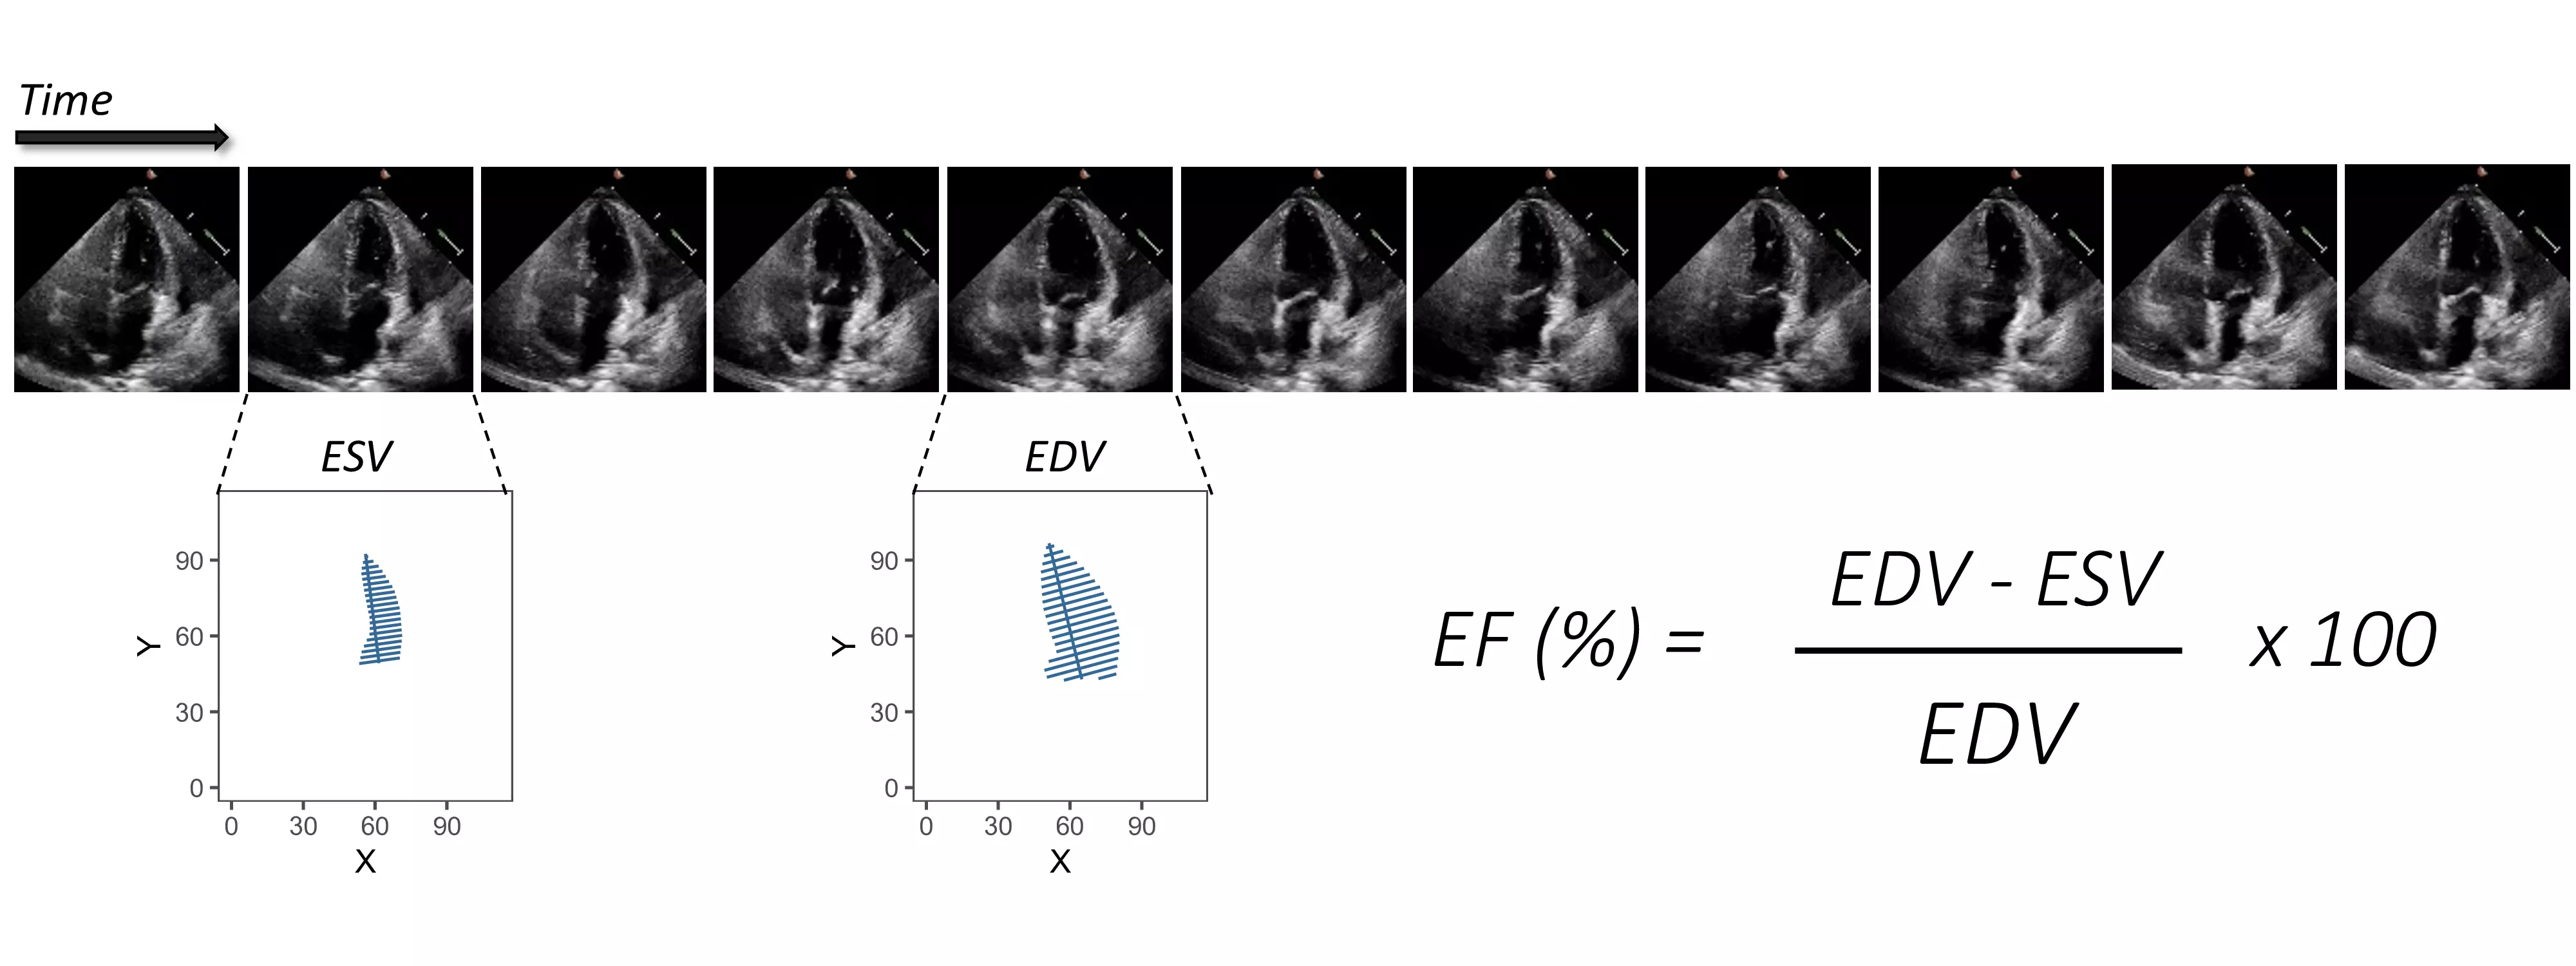
\includegraphics[scale=0.085]{images/esqueleto2.png}
    \caption{Ejemplificación del esqueleto formado en un par de fotogramas.~\cite{ref_url1}.}\label{fig:imagen1}
\end{figure}

Posteriormente, se realizó un gráfico de los puntos para generar una visión gráfica de su distribución en el plano cartesiano. Aunque en la figura número dos se muestran los resultados, se puede observar que los ventrículos están invertidos; esto se debe a la disposición del eje y para un fotograma de video cuyo valor máximo se encuentra en el origen del eje x.

\begin{figure}
    \centering
    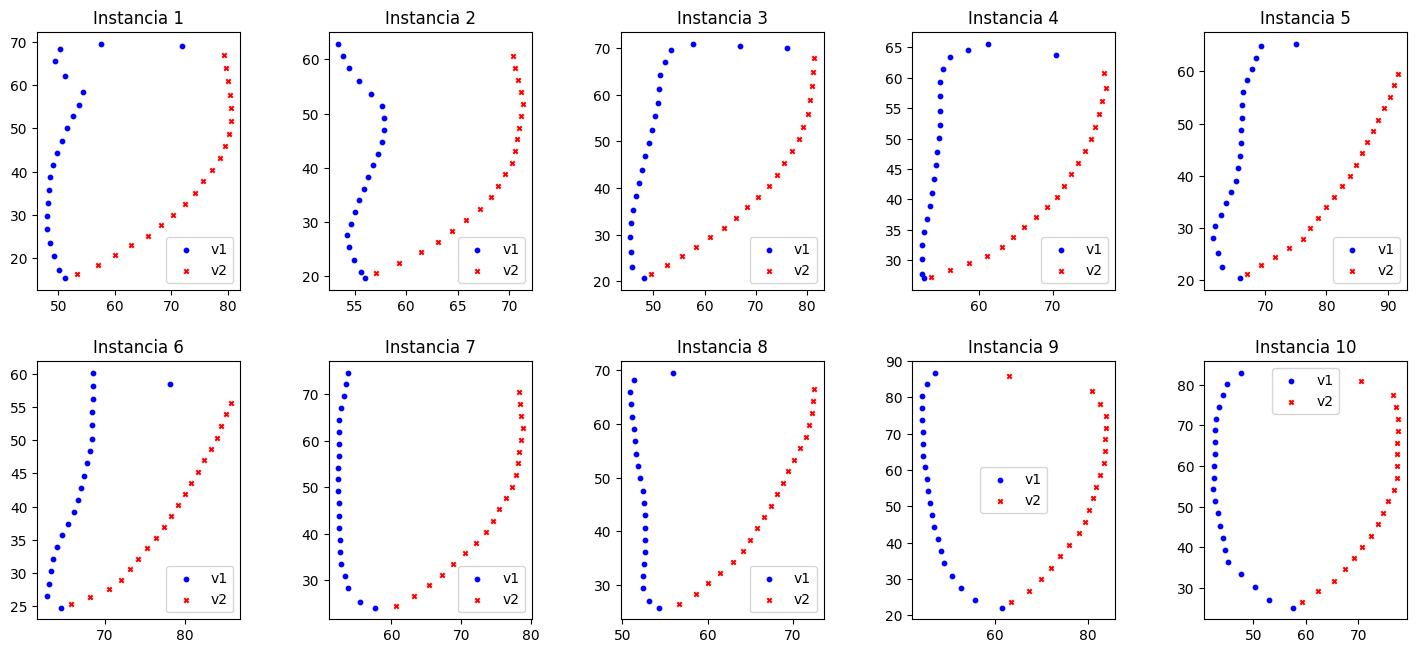
\includegraphics[scale=0.32]{images/Graficas.png}
    \caption{Gráfias con la distribución de puntos de 10 fotogramas seleccionados al azar.}\label{fig:imagen1}
\end{figure}


Una vez analizada la información proporcionada por el conjunto de datos, se procedió a desarrollar una estrategia para almacenarla y facilitar su consulta a lo largo de todo el proceso de ejecución y pruebas. Esto llevó al equipo a estructurar una clase que pudiera almacenar el nombre del archivo de vídeo, los fotogramas seleccionados y arreglos que contienen los puntos de las fronteras del ventrículo izquierdo.

Una vez concluido este proceso, se avanzó en la generación de las máscaras. Sin embargo, se presentó un reto con el segmento de recta transversal del esqueleto, ya que la función para rellenar el área requería que los puntos estuvieran ordenados en el sentido de las manecillas del reloj. Esto llevó a la creación de un algoritmo que permitiera identificar esos puntos atípicos y reacomodarlos. Como resultado, se obtuvieron las máscaras binarias que conformarían el conjunto de validación para los entrenamientos de los modelos.

\begin{figure}
    \centering
    \begin{subfigure}{0.45\linewidth}
        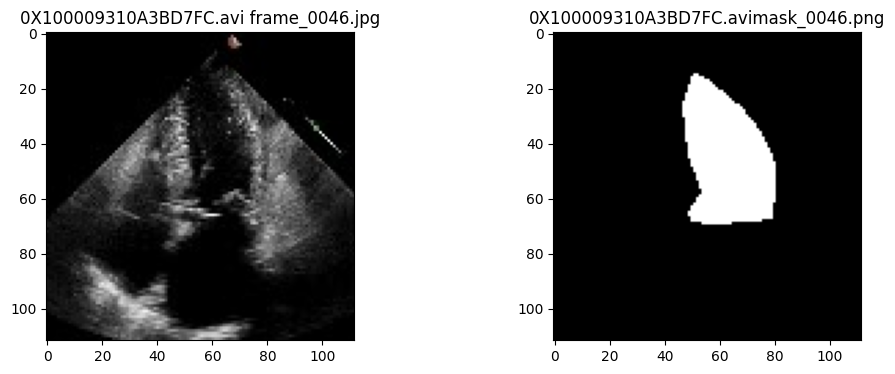
\includegraphics[scale= 0.205]{images/Mask1.png}
    \end{subfigure}
    \begin{subfigure}{0.45\linewidth}
        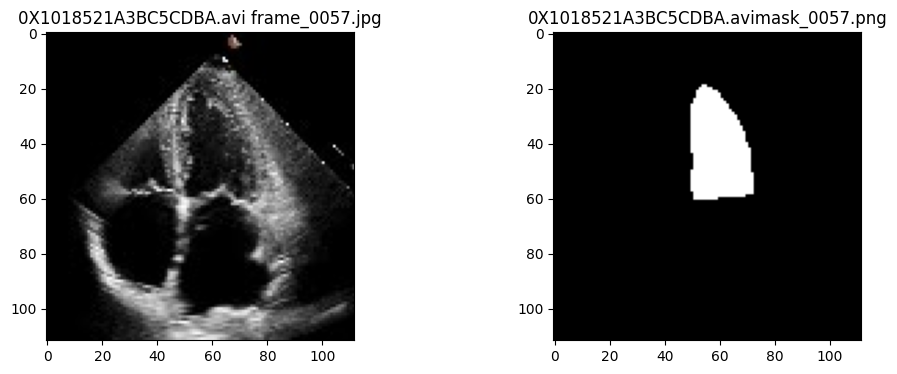
\includegraphics[scale= 0.205]{images/Mask2.png}
    \end{subfigure}
    \caption{Máscaras binarias generadas para el conjunto de validación.}
\end{figure}

\section{Metodología}

\subsection{Modelo de predicción de máscaras}

Una vez generadas las instancias de la clase y las máscaras para validar las predicciones, se procedió a crear un modelo U-NET para iniciar los primeros entrenamientos y realizar las predicciones. Es relevante destacar que se empleó una red neuronal convolucional en los entrenamientos. Estas redes constan de tres tipos principales de capas:

\begin{figure}
    \centering
    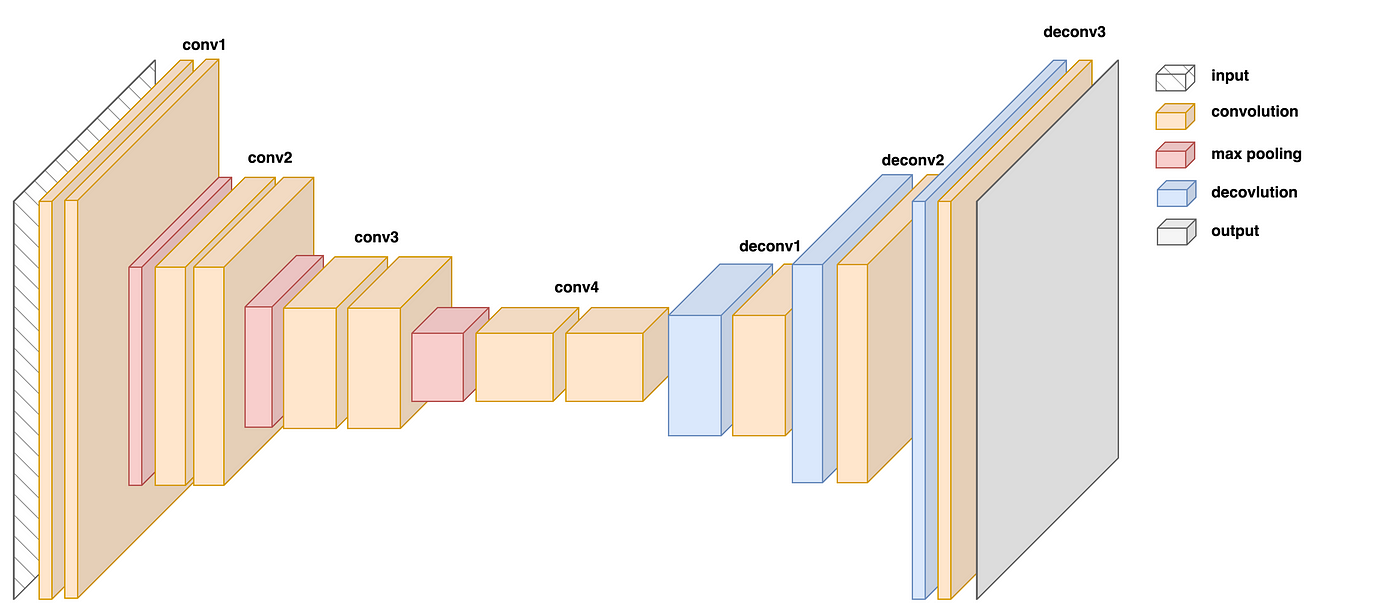
\includegraphics[scale=0.2]{images/red.png}
    \caption{Representación gráfica de una Red Neuronal Convolucional.}\label{fig:imagen1}
\end{figure}

\begin{itemize}
    \begin{itemize}
        \item \textbf{Capas convolucionales}: Estas capas reducen el tamaño de las imágenes y, a través de filtros, ayudan a reconocer patrones simples, curvas y ejes en las imágenes.
        \item \textbf{Capas de agrupación máxima}: Estas capas agrupan los píxeles que tienen mayor importancia, generalmente aquellos más brillantes.
        \item \textbf{Capas de deconvolución}: Estas capas aumentan la resolución de la imagen para devolverla a su resolución original o incrementarla en el proceso.
    \end{itemize}
\end{itemize}

Este tipo de modelos reciben como entrada un grid de números, que es la forma en que la computadora procesa imágenes. Comprender la estructura de las redes neuronales convolucionales permite entender lo que sucede internamente cuando se ejecutan los modelos para realizar diversas predicciones. Así mismo, es importante resaltar que el uso de un modelo U-net en este caso, se debe a que ha demostrado ser muy eficaz para el análisis de imágenes realcionadas con el sector salud.

\section{Experimentos}

\subsection{Modelo de predicción de máscaras}

En el proceso de validación y pruebas del primer modelo de predicciones, se tomó la decisión de evaluar su rendimiento utilizando un conjunto de datos extremadamente reducido, compuesto únicamente por 10 fotogramas. Es relevante subrayar que la primera red convolucional, objeto de este análisis, contaba con 5 capas de convolución. Durante las pruebas, se procedió a realizar cambios en las funciones de pérdida para evaluar su impacto en el desempeño del modelo.

Al realizar un análisis preliminar de los resultados obtenidos, se observó que, aunque la precisión (accuracy) era considerablemente alta, las máscaras resultantes presentaban deficiencias notables. Ante este panorama, se decidió llevar a cabo un aumento en la cantidad de datos utilizados para el entrenamiento, con la expectativa de mejorar el rendimiento del modelo. Si bien esta estrategia logró cierta mejora en las predicciones, se mantenía el objetivo de obtener un resultado más nítido y óptimo en términos de segmentación de imágenes.

Este escenario condujo a la construcción de un nuevo modelo, concebido para ser más robusto y entrenado con la mayor cantidad posible de imágenes. En nuevo modelo tuvo un total de 10 capas y al considerar que se seleccionaron 2 fotogramas de todo el conjunto de datos, la distribución de clases se organizó de la siguiente manera: 14,920 imágenes para entrenamiento, 2,552 para pruebas y 2,574 para validación, totalizando así 20,060 imágenes segmentadas. La estrategia implementada no solo proporcionó un resultado óptimo sino que también sentó las bases para el desarrollo del modelo de landmarks. En las figura 5 se muestra la máscara resultante de cada una de las pruebas realizadas. 

\begin{figure}
    \centering
    \begin{subfigure}{0.45\linewidth}
        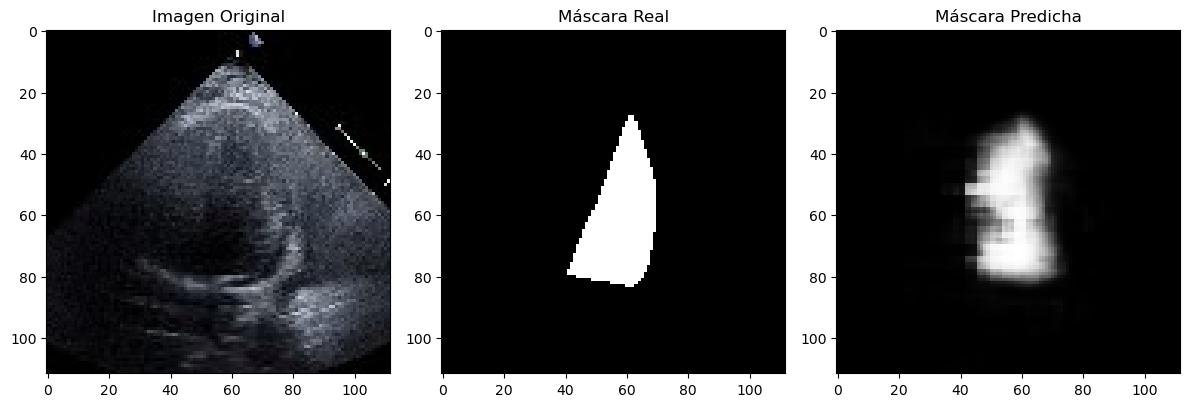
\includegraphics[scale= 0.18]{images/Mask_pred1.png}
        \caption{Predicción con modelo de 5 capas.}
    \end{subfigure}
    \begin{subfigure}{0.45\linewidth}
        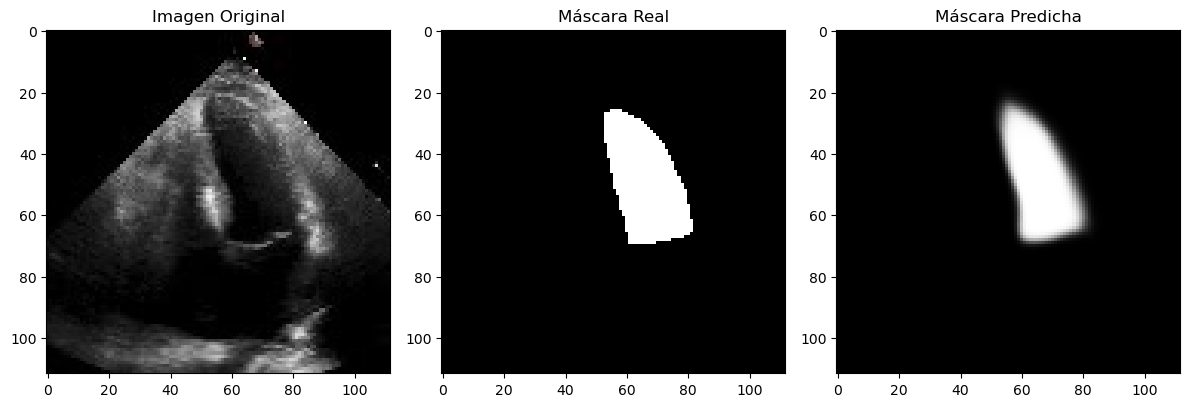
\includegraphics[scale= 0.18]{images/Mask_prediction1.png}
        \caption{Predicción con modelo de 10 capas.}
    \end{subfigure}
    \caption{Máscaras binarias generadas con los modelos de prueba (a) y final (b).}
\end{figure}

\subsection{Modelo de predicción de landmarks}

Antes de abordar el proceso de experimentación de este modelo, es crucial destacar el concepto de landmark, que representa un punto de relevancia estratégicamente posicionado con un propósito específico. En este caso, los landmarks se implementaron con el fin de predecir el perímetro correspondiente al ventrículo izquierdo en los ecocardiogramas. Para lograrlo, fue necesario realizar un preprocesamiento de las imágenes previamente seleccionadas, convirtiéndolas en un grid numérico o matríz para destacar los contornos de la máscara con los píxeles de la imagen , y posteriormente identificar los puntos de mayor relevancia para cerrar el perímetro ventricular.

La estrategia adoptada consistió en identificar 7 puntos distribuidos de la siguiente manera: uno en la posición más alta del área ventricular, 2 en las esquinas inferiores y 2 a cada lado de las paredes ventriculares. Una vez generado este mapeo, se procedió a crear un mapa de calor (heatmap) para visualizar la relevancia de estos puntos. Estos nuevos requerimientos desencadenaron un ajuste en el modelo, ya que su entrada pasó a ser la distribución de probabilidades gaussianas del contorno de la máscara ventricular y como salida se tendrían 7 canales, uno por cada punto a predecir. A diferencia del modelo anterior, que tenía una única salida binaria.

Considerados los ajustes se realizó una revisión de cómo se comportaban los landmarks. La figura 6 presenta los mapas de calor de una máscara de prueba, junto con una representación gráfica de la probabilidad gaussiana radial de los puntos y su distribución sobre el perímetro de la máscara.

\begin{figure}
    \centering
    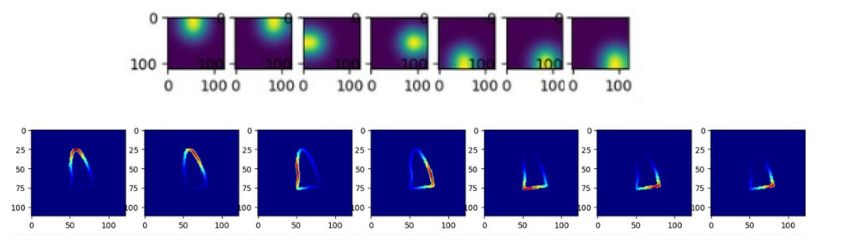
\includegraphics[scale=1.5]{images/landmarks.png}
    \caption{Mapas de calor en el plano y sobre el perímetro ventricular.}\label{fig:imagen1}
\end{figure}

Una vez validado que el algoritmo estaba identificando los landmarks de manera adecuada, se detonó el entrenamiento del modelo. Sin embargo, se encontró una limitación en la memoria disponible para realizar pruebas, lo que llevó a la decisión de reducir las capas del modelo con el objetivo de limitar el procesamiento necesario. Después de llevar a cabo diversas pruebas, se optó por un modelo de 5 capas, similar al utilizado en la primera etapa de pruebas del modelo anterior. A pesar de esta reducción, los resultados obtenidos fueron satisfactorios. La imagen número 7 muestra la comparación de un ecocardiograma seleccionado, el perímetro que se buscaba predecir y el resultado obtenido por el modelo. Este análisis visual permite evaluar la efectividad del modelo en la predicción precisa de los landmarks y, por ende, del perímetro ventricular en los ecocardiogramas.

\begin{figure}
    \centering
    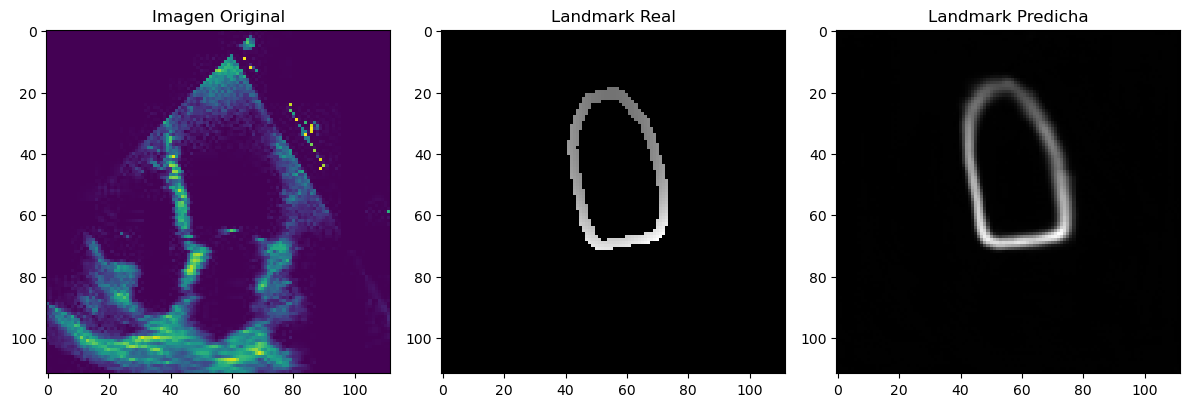
\includegraphics[scale=0.3]{images/Landmark_prediction1.png}
    \caption{Predicción del modelo final de landmarks.}\label{fig:imagen1}
\end{figure}

Al concluir el proceso de experimentación, se seleccionó una estrategia para medir la precisión del modelo. Para ello, se utilizó la función Structural Similarity (SSIM) con el propósito de comparar el área predicha por los modelos con el área real definida en las máscaras de validación. Esta función aplica un filtro a la máscara predicha y la compara con la máscara real, proporcionando un porcentaje de similitud como resultado. En la Tabla 2 se presentan los porcentajes de similitud obtenidos por los modelos, ofreciendo una métrica cuantitativa para evaluar la calidad de las predicciones.

\vspace{-1em} % Ajusta la distancia vertical negativamente
\begin{table}
    \centering
    \begin{tabular}{lccc}
    \toprule
    Modelo & Porcentaje de simulitud \\
    \midrule
    Máscarás & 90.54\\
    Landmarks & 85.31\\
    \bottomrule
    \end{tabular}
    \vspace{1em} % Ajusta la distancia vertical negativamente
    \caption{Resultados de similitud}\label{tab2}
\end{table}

\vspace{-1em} % Ajusta la distancia vertical negativamente

Después de entrenar los modelos, se llevaron a cabo evaluaciones mediante 15 predicciones utilizando imágenes externas al conjunto de datos de prueba. El objetivo era analizar el comportamiento del modelo frente a ecocardiogramas que presentaran más ruido o no fueran tan nítidos como las imágenes utilizadas durante el entrenamiento. Sorprendentemente, y en contraste con los resultados anteriores, se observó que el modelo de landmarks mostró una eficiencia superior para este conjunto de imágenes externas, como se ilustra en la figura número 8. Este hallazgo resalta la capacidad del modelo para generalizar su desempeño a datos más diversos y ruidosos.

\begin{figure}
    \centering
    \begin{subfigure}{0.45\linewidth}
        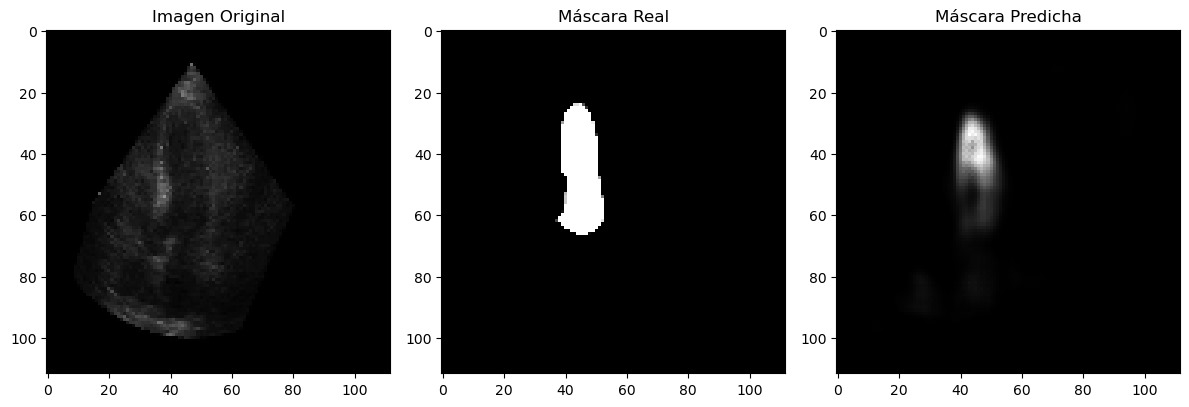
\includegraphics[scale= 0.18]{images/mask_test.jpg}
        \caption{Prueba con modelo de máscaras.}
    \end{subfigure}
    \begin{subfigure}{0.45\linewidth}
        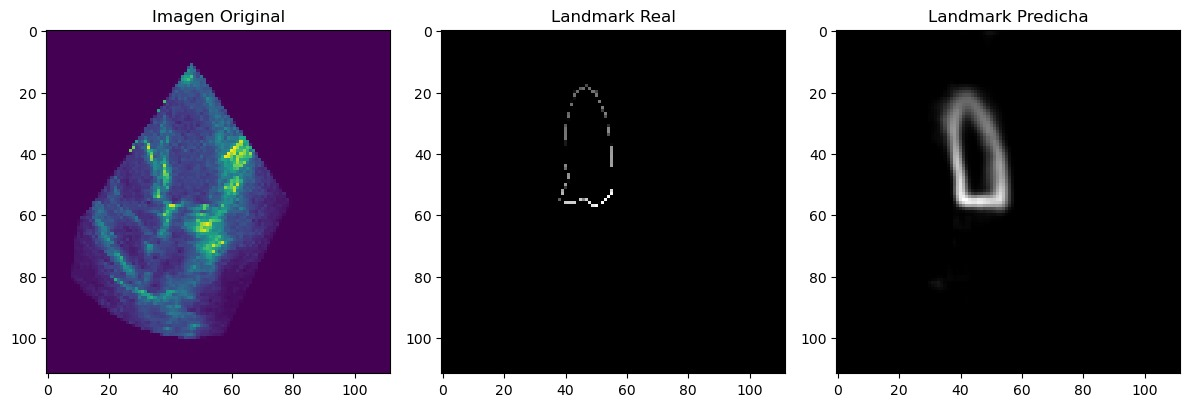
\includegraphics[scale= 0.18]{images/landmark_test.jpg}
        \caption{Prueba con modelo de landmarks.}
    \end{subfigure}
    \caption{Predicciones obtenidas. Máscaras(a) Landmarks (b).}
\end{figure}


\section{Resultados}

Al concluir todo el proceso de experimentación, se tomó la decisión de presentar de manera gráfica la distribución de resultados de similitud de ambos modelos. Aunque se proporcionó un resultado numérico anteriormente, es relevante identificar la distribución de la similitud en todo el segmento de prueba. En la figura siguiente, se muestran los histogramas tanto para el modelo de máscaras como para el modelo de landmarks.

\begin{figure}
    \centering
    \begin{subfigure}{0.45\linewidth}
        \centering
        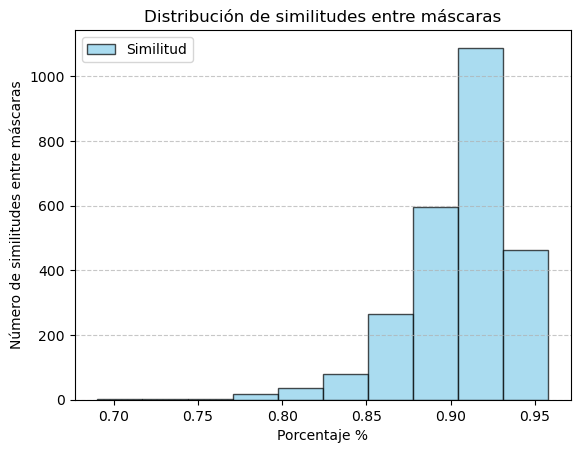
\includegraphics[scale= 0.3]{images/histograma_mascaras.png}
        \caption{Histograma de resultados (máscaras).}
    \end{subfigure}
    \begin{subfigure}{0.45\linewidth}
        \centering
        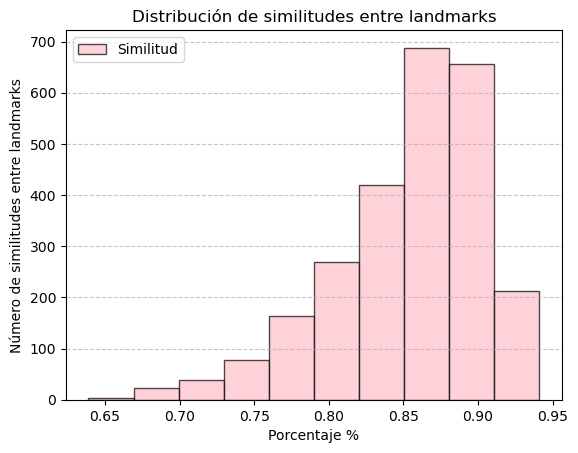
\includegraphics[scale= 0.3]{images/histograma_landmarks.png}
        \caption{Histograma de resultados (landmarks).}
    \end{subfigure}
    \caption{Predicciones obtenidas con imágenes del conjunto de prueba. Máscaras(a) Landmarks (b).}
\end{figure}

A pesar de que ambos modelos arrojaron resultados muy buenos, se puede observar que el modelo de máscaras tuvo un desempeño ligeramente superior en el conjunto de datos original. No obstante, el proceso de experimentación dejó en claro que el modelo de máscaras destaca en comparación por la nitidez de los ecocardiogramas analizados. Por esta razón, se considera esencial presentar también los histogramas de similitud obtenidos en la fase de pruebas que involucró imágenes externas a los conjuntos de prueba.

\begin{figure}
    \centering
    \begin{subfigure}{0.45\linewidth}
        \centering
        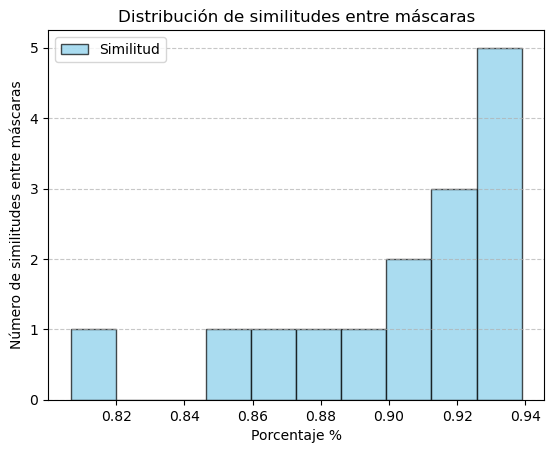
\includegraphics[scale= 0.3]{images/histograma_exp_mascaras.png}
        \caption{Histogramas de resultados del conjunto de imágenes de prueba del dataset.}
    \end{subfigure}
    \begin{subfigure}{0.45\linewidth}
        \centering
        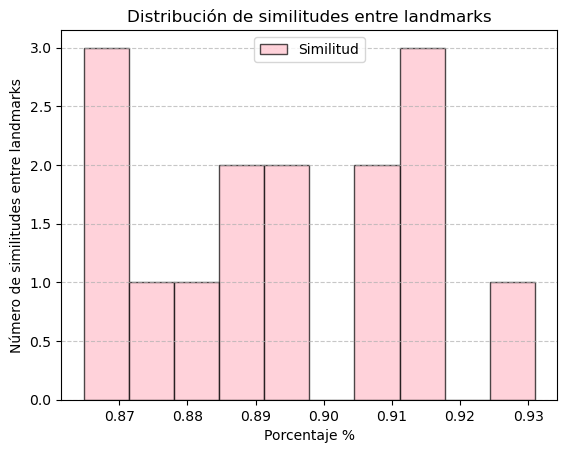
\includegraphics[scale= 0.3]{images/histograma_exp_landmarks.png}
        \caption{Histograma de resultados de prueba (landmarks).}
    \end{subfigure}
    \caption{Histogramas de resultados del conjunto de imágenes externo al dataset.}
\end{figure}

Nuevamente, se observa que el modelo de máscaras mostró un porcentaje de similitud más alto en este conjunto de pruebas. Sin embargo, es importante señalar que los resultados visuales fueron significativamente mejores con el modelo de landmarks y dada la naturaleza del problema se priorizan los resulatdos visuales que los numéricos. Esta disparidad tiene su origen en la limitada cantidad de imágenes utilizadas para este proceso. Para futuras mejoras, se ha identifiado el considerar la inclusión de imágenes con menos nitidez en el conjunto de entrenamiento para que el modelo adquiera la capacidad de identificar la cavidad ventricular izquierda incluso en imágenes con más ruido.

\section{Conclusiones}

Los resultados obtenidos en este trabajo lograron generar y comparar dos modelos de inteligencia artificial diseñados para segmentar el ventrículo izquierdo del corazón a partir de imágenes de ecocardiogramas. Este proyecto resultó de vital importancia, no solo para establecer los conceptos fundamentales de las estructuras de modelos de redes neuronales convolucionales, su funcionamiento y los fundamentos matemáticos que permiten comprender su operación, sino también como un medio para entender la aplicabilidad de la inteligencia artificial en campos como la medicina.

Además de los aspectos técnicos, este proyecto abordó de manera consciente la ética vinculada al uso y manejo de datos sensibles. Pues implica el uso de imágenes que representan las condiciones de salud de muchas personas, destacando la importancia de ser conscientes de la relevancia del análisis de datos en la actualidad. Es fundamental aprender a utilizar información de acceso público, cumplir con los lineamientos establecidos por las instituciones que facilitan el acceso a estos datos, y comprender la importancia de que estos estén anonimizados para su uso y análisis. Este enfoque ético es esencial en el desarrollo de proyectos de inteligencia artificial en todos los ámbitos.

Finalmente, se aplicaron conceptos como el uso de cómputo en la nube, que se convirtió en el medio para almacenar las diversas imágenes generadas por el modelo y los datos de entrenamiento, prueba y validación. Esto garantizó que los miembros del equipo tuvieran acceso a ellas para realizar pruebas de manera remota. Además, se destacó la importancia del uso de conocimientos estadísticos para evaluar el rendimiento del modelo. La combinación de estos elementos permitió poner en práctica y consolidar los diversos contenidos aprendidos en clase, abarcando desde el manejo de datos hasta la construcción y evaluación efectiva de modelos de inteligencia artificial.

\section{Conclusiones Individuales}

\subsection*{Andrés Alejandro Guzmán González}

Con el desarrollo de este trabajo, tuve la oportunidad de aplicar los conocimientos adquiridos en clase, comprendiendo a fondo cómo la inteligencia artificial puede ser una herramienta transformadora en diversos aspectos de la vida cotidiana, especialmente en la optimización de procesos. En particular, encuentro muy enriquecedora la situación problema qué va de automatizar el proceso de segmentación del ventrículo izquierdo mediante la implementación de modelos de inteligencia artificial y visión computacional. Así mismo, la aplicación de conceptos estadísticos para la evaluación de los rendimientos de un modelo de inteligencia artificial, estrategias de administración, almacenamiento y control de grandes cantidades de datos (Big Data), y la aplicación de estrategias de almacenamiento en la nube para eficientar procesos de consulta de información y/o datos.

Este proyecto me ha proporcionado una visión más clara sobre cómo la tecnología puede ser un medio para mejorar significativamente la calidad de vida de las personas. Pero también sobre la importancia de tener presente la ética con el manejo de datos, este reto presentaba el uso de imágenes sensibles y confidenciales que podrían reflejar el estado de salud de muchas personas, es por ello qué ser conscientes de las diferentes normativas para el uso de datos es indispensable para el desarrollo de cualquier proyecto tecnológico no solo los de inteligencia artificial.Considero que este proyecto fue tanto retador como fascinante, ya que me permitió explorar la estructuración de diferentes modelos de inteligencia artificial y conocer diversas estrategias que actualmente la industria aplica para contribuir positivamente a la sociedad. Este proceso no solo ha mejorado mi dominio práctico de los conceptos de la concentración; también ha detonado mi interés por seguir explorando aplicaciones de la inteligencia artificial para resolver problemas cotidianos.

\subsection*{Ernesto Reynoso Lizárraga}

A lo largo de este proyectó aprendí varias acerca de los modelos de inteligencia artificial y también sobre las problemáticas que se enfrenta la industria hoy en día y que se busca resolver con dichos modelos. Con los resultados de nuestro modelo puedo concluir que realizar un modelo de inteligencia artificial no es fácil y hay muchos factores a tener en cuenta, tales como los datos con los que vas a trabajar, los hiperparametros, la efectividad, el tiempo de ejecución, hasta otros factores no propios del modelo como el equipo con el que estas trabajando. También cabe mencionar que no existe una forma de hacer el modelo ideal más allá de la aproximación y la prueba y error, y que como observamos en los resultados, el modelo puede resolver eficientemente el problema si lo ajustas al conjunto de datos con el que trabajas, pero puede no ser lo ideal cuando se intenta predecir imágenes de un conjunto de datos distinto. Para finalizar quiero decir que se debe de ser muy consciente y responsable sobre los datos con los que se están trabajando ya que dichos datos, aunque estén destinados para la experimentación y el estudio, siguen siendo datos reales de personas, por lo que se debe de tener cierto criterio al trabajar con ellos.

\subsection*{Joel Isaias Solano Ocampo}

La solución reto a conllevar durante estos dos bloques de desarrollo en segunda mitad de la concentración de Inteligencia artificial avanzada para la ciencia de datos fue más que solo retadora. Estuvo llena de obstáculos, llena de incógnitas y sobre todo, mucho aprendizaje de por medio. Como equipo, siento que llegamos a tener muchas dificultades en determinados procesos técnicos al momento de tratar de implementar ciertas soluciones algorítmicas o de complejidad tanto de hardware como de software lo que llegó a detener en determinados momentos el flujo constante que solíamos tener de trabajo. De aquí puede también mencionar que se deriva de muchas dudas respecto a qué soluciones podríamos tratar de aproximarnos para solventar dichos obstáculos, cuales podrian ser las mas efectivas, como llegaron dichas soluciones a impactar en toda la implementación y si dicha solución no sería solo el generador de mayores dificultades que remedios para el objetivo deseado. Algo que definitivamente nos terminó marcando como equipo, individuos y compañeros fueron los aprendizajes que obtuvimos durante la implementación del reto, ya que estábamos adentrándonos en una rama de conocimiento de nuestra carrera que es nueva y compleja para todos nosotros. Además, se trató de una concentración cuyo objetivo es precisamente buscar un tipo de especialización en el área para que más adelante nos podamos seguir especializando en el área una vez concluya la misma e inclusive una vez terminemos la carrera profesional y decidimos adentrarnos en el tema ya sea por medio de la industria, la investigación o algún otro medio posible en donde podamos ver reflejado nuestro trabajo. Para terminar de hablar, me gustaría decir que me termino agradando mucho lo que se terminó logrando con este reto de tan gran impacto, me sorprendió mucho cómo a pesar de seguir siendo estudiantes de universidad y de ser esta nuestra primera aproximación a la materia, tuvimos la oportunidad de mostrar nuestros resultados a una empresa de reconocimiento y pronombre mundial en el área de la inteligencia artificial. Me termino llevando de este reto y de esta concentración las ganas de seguir aprendiendo de este campo tan amplio que es la inteligencia artificial para seguir desarrollándome de manera profesional y así alcanzar objetivos que si bien, aún no me he podido plantear aun, se que se aproximarán eventualmente.


\subsection*{Tania Sayuri Guizado Hernandez}

En desarrollo de este proyecto, a partir de nuestro dataset EchoNet-Dynamic Cardiac Ultrasound, el equipo fue capaz de emplear habilidades técnicas para el procesamiento de imágenes, aplicación de algoritmos de aprendizaje profundo, así como también una comprensión sólida de la ética en la investigación médica y el cumplimiento normativo. Quisiera resaltar especialmente que nos propusimos investigar cómo nuestro conjunto de datos establece de manera clara en sus condiciones de uso la restricción de distribución y la garantía de que su utilización esté destinada exclusivamente a fines de investigación no comerciales. Asimismo, en lo que respecta a la anonimización, reconocemos que la integridad y privacidad de los datos se preservan conforme a lo estipulado en su página oficial. Esta información desempeñó un papel esencial en nuestro proyecto porque atribuyó a respaldar la transparencia y la trazabilidad en la gestión de datos sensibles. Por otro lado, en la aplicación de modelos U-Net obtuvimos una nueva perspectiva, porque durante el proceso fuimos descubriendo la necesidad e importancia de no solo familiarizarse con  arquitecturas de redes neuronales y dominio de técnicas de aprendizaje profundo, sino el también de cultivar una apreciación crítica de los principios médicos subyacentes. Al enfrentarnos a desafíos significativos y una complejidad inherente en la obtención de máscaras precisas del ventrículo izquierdo, así como los posibles rangos para asignar a una landmark, en la superación de estas complejidades mediante una integración eficaz de avanzadas técnicas de aprendizaje profundo, aspiramos a entender que esta implementación no solo facilitará una segmentación más precisa, sino que también contribuirá de manera sustancial a una interpretación más refinada de las imágenes cardíacas en un escenario real del ámbio médico a lo que atribuirá en diagnosticos y tratamientos eficientes. Con esta valiosa experiencia, logré observar cómo la sinergia entre la tecnología de vanguardia y la medicina demuestra que la aplicación efectiva de modelos de aprendizaje profundo puede generar un impacto notable en la mejora de la atención médica, y quizá en cualquier campo diferente al ámbito medicinal.
\vspace{5em} % Ajusta la distancia vertical negativamente

% ---- Bibliography ----
%
% BibTeX users should specify bibliography style 'splncs04'.
% References will then be sorted and formatted in the correct style.
%
% \bibliographystyle{splncs04}
% \bibliography{mybibliography}
%
\begin{thebibliography}{99}

%\bibitem{ref_book1}
%Geron, A.: Hands-On Machine Learning with Scikit-Learn and TensorFlow: 
%Concepts, Tools, and Techniques to Build Intelligent Systems. O'Reilly (2019)

\bibitem{ref_url1}
EchoNet-Dynamic.(2020). \textit{Standford University}. Disponible en: 
\url{https://echonet.github.io/dynamic/}. 
Accedido en Septiembre de 2023.

\bibitem{ref_url2}
Definición de cardiopatía. (s.f.). \textit{Instituto Nacional del cancer}. Disponible en: 
\url{https://www.cancer.gov/publications/dictionaries/cancer-terms/def/heart-disease}. 
Accedido en noviembre de 2023.

\bibitem{ref_url4}
EchoNet-Dynamic.[imagen] (2020). \textit{Standford University}. Disponible en: 
\url{https://echonet.github.io/dynamic/}. 
Accedido en Septiembre de 2023.


\bibitem{ref_url8}
Enfermedades cardiovasculares. (s.f.). \textit{Organización Mundial de la Salud}. Disponible en: 
\url{https://www.who.int/es/health-topics/cardiovascular-diseases#tab=tab_1}. 
Accedido en noviembre de 2023.


\end{thebibliography}
\end{document}
